\documentclass[journal,12pt,twocolumn]{IEEEtran}

\usepackage{setspace}
\usepackage{gensymb}
\singlespacing
\usepackage[cmex10]{amsmath}

\usepackage{amsthm}

\usepackage{mathrsfs}
\usepackage{txfonts}
\usepackage{stfloats}
\usepackage{bm}
\usepackage{cite}
\usepackage{cases}
\usepackage{subfig}

\usepackage{longtable}
\usepackage{multirow}

\usepackage{enumitem}
\usepackage{mathtools}
\usepackage{steinmetz}
\usepackage{tikz}
\usepackage{circuitikz}
\usepackage{verbatim}
\usepackage{tfrupee}
\usepackage[breaklinks=true]{hyperref}
\usepackage{graphicx}
\usepackage{tkz-euclide}

\usetikzlibrary{calc,math}
\usepackage{listings}
    \usepackage{color}                                            %%
    \usepackage{array}                                            %%
    \usepackage{longtable}                                        %%
    \usepackage{calc}                                             %%
    \usepackage{multirow}                                         %%
    \usepackage{hhline}                                           %%
    \usepackage{ifthen}                                           %%
    \usepackage{lscape}     
\usepackage{multicol}
\usepackage{chngcntr}

\DeclareMathOperator*{\Res}{Res}

\renewcommand\thesection{\arabic{section}}
\renewcommand\thesubsection{\thesection.\arabic{subsection}}
\renewcommand\thesubsubsection{\thesubsection.\arabic{subsubsection}}

\renewcommand\thesectiondis{\arabic{section}}
\renewcommand\thesubsectiondis{\thesectiondis.\arabic{subsection}}
\renewcommand\thesubsubsectiondis{\thesubsectiondis.\arabic{subsubsection}}


\hyphenation{op-tical net-works semi-conduc-tor}
\def\inputGnumericTable{}                                 %%

\lstset{
%language=C,
frame=single, 
breaklines=true,
columns=fullflexible
}
\begin{document}

\newcommand{\BEQA}{\begin{eqnarray}}
\newcommand{\EEQA}{\end{eqnarray}}
\newcommand{\define}{\stackrel{\triangle}{=}}
\bibliographystyle{IEEEtran}
\raggedbottom
\setlength{\parindent}{0pt}
\providecommand{\mbf}{\mathbf}
\providecommand{\pr}[1]{\ensuremath{\Pr\left(#1\right)}}
\providecommand{\qfunc}[1]{\ensuremath{Q\left(#1\right)}}
\providecommand{\sbrak}[1]{\ensuremath{{}\left[#1\right]}}
\providecommand{\lsbrak}[1]{\ensuremath{{}\left[#1\right.}}
\providecommand{\rsbrak}[1]{\ensuremath{{}\left.#1\right]}}
\providecommand{\brak}[1]{\ensuremath{\left(#1\right)}}
\providecommand{\lbrak}[1]{\ensuremath{\left(#1\right.}}
\providecommand{\rbrak}[1]{\ensuremath{\left.#1\right)}}
\providecommand{\cbrak}[1]{\ensuremath{\left\{#1\right\}}}
\providecommand{\lcbrak}[1]{\ensuremath{\left\{#1\right.}}
\providecommand{\rcbrak}[1]{\ensuremath{\left.#1\right\}}}
\theoremstyle{remark}
\newtheorem{rem}{Remark}
\newcommand{\sgn}{\mathop{\mathrm{sgn}}}
\providecommand{\abs}[1]{\vert#1\vert}
\providecommand{\res}[1]{\Res\displaylimits_{#1}} 
\providecommand{\norm}[1]{\lVert#1\rVert}
%\providecommand{\norm}[1]{\lVert#1\rVert}
\providecommand{\mtx}[1]{\mathbf{#1}}
\providecommand{\mean}[1]{E[ #1 ]}
\providecommand{\fourier}{\overset{\mathcal{F}}{ \rightleftharpoons}}
%\providecommand{\hilbert}{\overset{\mathcal{H}}{ \rightleftharpoons}}
\providecommand{\system}{\overset{\mathcal{H}}{ \longleftrightarrow}}
	%\newcommand{\solution}[2]{\textbf{Solution:}{#1}}
\newcommand{\solution}{\noindent \textbf{Solution: }}
\newcommand{\cosec}{\,\text{cosec}\,}
\providecommand{\dec}[2]{\ensuremath{\overset{#1}{\underset{#2}{\gtrless}}}}
\newcommand{\myvec}[1]{\ensuremath{\begin{pmatrix}#1\end{pmatrix}}}
\newcommand{\mydet}[1]{\ensuremath{\begin{vmatrix}#1\end{vmatrix}}}
\numberwithin{equation}{subsection}
\makeatletter
\@addtoreset{figure}{problem}
\makeatother
\let\StandardTheFigure\thefigure
\let\vec\mathbf
\renewcommand{\thefigure}{\theproblem}
\def\putbox#1#2#3{\makebox[0in][l]{\makebox[#1][l]{}\raisebox{\baselineskip}[0in][0in]{\raisebox{#2}[0in][0in]{#3}}}}
     \def\rightbox#1{\makebox[0in][r]{#1}}
     \def\centbox#1{\makebox[0in]{#1}}
     \def\topbox#1{\raisebox{-\baselineskip}[0in][0in]{#1}}
     \def\midbox#1{\raisebox{-0.5\baselineskip}[0in][0in]{#1}}
\vspace{3cm}
\title{AI1103-Assignment 2}
\author{Kodavanti Rama Sravanth, CS20BTECH11027}
\maketitle
\newpage
\bigskip
\renewcommand{\thefigure}{\theenumi}
\renewcommand{\thetable}{\theenumi}
Download all python codes from 
\begin{lstlisting}
https://github.com/Sravanth-k27/AI1103/tree/main/Assignment-2/codes
\end{lstlisting}
%
and latex-tikz codes from 
%
\begin{lstlisting}
https://github.com/Sravanth-k27/AI1103/tree/main/Assignment-2/Assignment-2.tex
\end{lstlisting}
\section*{Question(Gate EC 55):}
 Let $X_1$ be an exponential random variable
with mean 1 and $X_2$ a gamma random variable
with mean 2 and variance 2. If $X_1$ and $X_2$ are
independently distributed,then $P(X_1 < X_2)$ is equal to
\section*{Solution(Gate EC 55):}
\begin{enumerate}
    \item Given that $X_1$ is an exponential random variable. Let the P.D.F of $X_1$ be
    \begin{align}
    P_{X_1}(x_1)=
        \begin{cases}
        \lambda e^{-\lambda x_1} & x \geq 0\\
        0 & x<0
        \end{cases}
    \end{align}
    \begin{align}
    \text{ As mean}=\lambda\\
     \text{ Given that mean}=1\\
     \text{so } \lambda=1
    \end{align} 
     The P.D.F of $X_1$ is:
    \begin{align}
       P_{X_1}(x_1)=
        \begin{cases}
        e^{-x_1} & x\geq 0\\
        0 & x<0
        \end{cases}
    \end{align}
    \item Given that $X_2$ is an gamma random variable.Let the P.D.F of $X_2$ be:
    \begin{align}
        P_{X_2}(x_2)=
        \begin{cases}
            \frac{a^b x_2^{b-1}e^{-ax_2}}{(b-1)!} & x\geq 0\\
            0 & x<0
        \end{cases}
    \end{align}
    \begin{align}
       \text{ Since mean}=\frac{b}{a}=2\label{eq:0.0.7}\\
         \text{Also,variance}=\frac{b}{a^2}=2\label{eq:0.0.8}
    \end{align}
  From \eqref{eq:0.0.7} and \eqref{eq:0.0.8}
  \begin{align}
      b=2,a=1
  \end{align}
  So, the P.D.F of $X_2$ is :
  \begin{align}
      P_{X_2}(x_2)=
      \begin{cases}
          x_2e^{-x_2} & x\geq 0 \\
          0 & x<0
      \end{cases}
  \end{align}
  Now we have to find $P(X_1<X_2)$\\
  \item Consider the random variable $Z=X_1-X_2$\\
  \text{Since}
  \begin{align}
 P(X_1<X_2)\implies P(X_1-X_2<0)
  \end{align}
  So, we have to find C.D.F of random variable Z for z $\leq 0$ i.e $P(z\leq 0)$\\ 
  \\C.D.F of random variable $Z=X_1-X_2$ for $z\leq 0$ :
\begin{align}
      F_Z(z) &=P(X_1-X_2 \leq z)\\
       &=\int_{-z}^\infty \int_{0}^{z+x_2}P_{X_1X_2}(x_1,x_2) dx_1 dx_2\\
       &=\int_{-z}^\infty \int_{0}^{z+x_2}P(x_1)P(x_2) dx_1dx_2\\
       &=\int_{-z}^\infty P(x_2)\brak{ \int_{0}^{z+x_2}P(x_1) dx_1} dx_2\\
       &=\int_{-z}^\infty x_2 e^{-x_2} \brak{\int_{0}^{z+x_2}e^{-x_1}dx_1}dx_2
  \end{align}
  Now for $F_Z(0)$
  \begin{align}
  \begin{split}
      F_Z(0)&=\int_{0}^\infty x_2 e^{-x_2} \brak{\int_{0}^{x_2}e^{-x_1}dx_1}dx_2\\
      &=\int_{0}^\infty x_2 e^{-x_2} \brak{1-e^{-x_2}}dx_2\\
      &=\int_{0}^\infty x_2 e^{-x_2}dx_2-\int_{0}^\infty x_2e^{-2x_2} dx_2\\
      &=1-\frac{1}{4}=\frac{3}{4}
      \end{split}
  \end{align}
  So, $P(X_1<X_2)=F_Z(0)=\frac{3}{4}$
\end{enumerate}

\begin{figure}[h]
    \begin{center}
    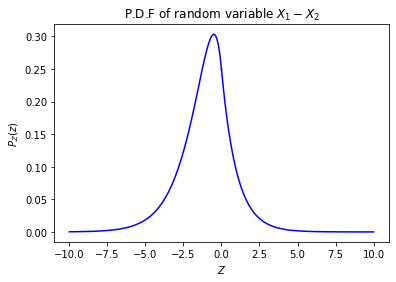
\includegraphics[scale=0.6]{figure-1.png}
    \end{center}
    \caption{P.D.F of Z}\label{Fig 1:}
\end{figure}
\begin{figure}[h]
   \begin{center}
    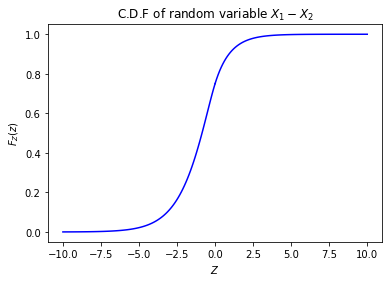
\includegraphics[scale=0.6]{figure-2.png}
    \end{center}
   \caption{C.D.F of Z}\label{Fig2:}
\end{figure}
\end{document}
